%*----------- SLIDE -------------------------------------------------------------
\begin{frame}[t]{Artigo de Referência} 
    \begin{center}
        \huge 
        Kinematic Modeling and Simulation of a SCARA Robot by Using Solid Dynamics and Verification by
        MATLAB/Simulink\\
        \!
        \\
        \normalsize
        M. S. Alshamasin, F. Ionescu, R. T. Al-Kasasbeh\\
        2009
        
    \end{center}
\end{frame}
%*----------- SLIDE -------------------------------------------------------------
\begin{frame}[c]{Robôs SCARA}
    \framesubtitle{Selective Compliance Articulated Robot Arm} 
    \begin{columns}
        % \column{.01\textwidth}
        \column{.01\textwidth}
        \column{.5\textwidth}

        \begin{figure}
            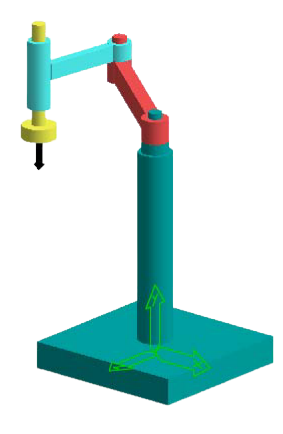
\includegraphics[trim = 0 0 0 0, clip, width=0.7\textwidth]{scara.png}
            %\caption{.}
        \end{figure}

        \column{.49\textwidth}
        \Large
        % São robôs manipuladores que possuem:
        \begin{itemize}
            \item Alta velocidade
            \item Alta precisão
            \item Melhor repetibilidade entre manipuladores
            \item 4 graus de liberdade
        \end{itemize}

    \end{columns}
   
%*----------- notes
    \note[item]{Notes can help you to remember important information. Turn on the notes option.}
\end{frame}
\begin{frame}[c]{Aplicações}

    \begin{columns}
        % \column{.01\textwidth}
        \column{.01\textwidth}
        \column{.49\textwidth}
        \begin{figure}
            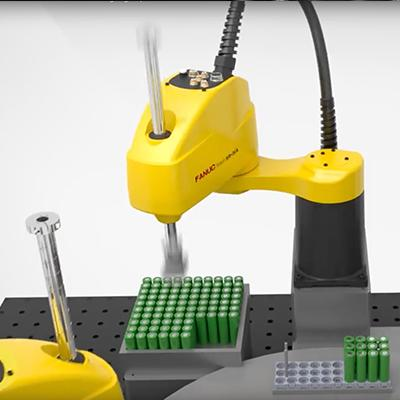
\includegraphics[trim = 0 0 0 0, clip, height=.88\textwidth]{FEA_Speed_assembly-Scara_400x400.jpg}
            %\caption{.}
        \end{figure}    
        % \includemovie{1cm}{1cm}{img07.gif}

        \column{.49\textwidth}
        \begin{figure}
            % 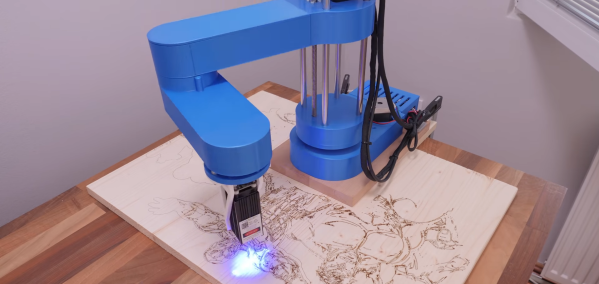
\includegraphics[trim = {5cm 0 5cm 0}, clip, height=.9\textwidth]{2021-08-26-19.png}
            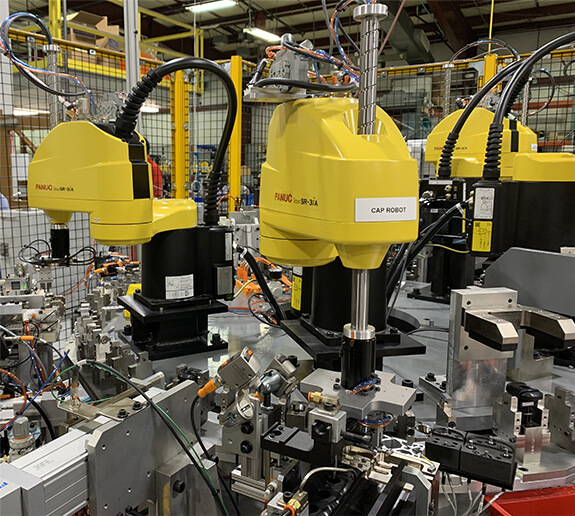
\includegraphics[trim = {0cm 0 0cm 0}, clip, height=.88\textwidth]{aplica2.jpg}
            %\caption{.}
        \end{figure}   
        \column{.01\textwidth}
    
    \end{columns}
    
%*----------- notes
    \note[item]{Notes can help you to remember important information. Turn on the notes option.}
\end{frame}
%*----------- SLIDE -------------------------------------------------------------
\begin{frame}[c]{A Importância das Simulações} 
    % \framesubtitle{Notação Denavit-Hartenberg}
    \begin{columns}
        \column{.01\textwidth}
        \column{.69\textwidth}
        As simulações possuem as seguintes vantagens:
        \begin{itemize}
            \item Fáceis de montar
            \item Baixo custo
            \item Resultados rápido
        \end{itemize}
        Poranto podem ser utilizadas para:
        \begin{itemize}
        \item Prever o comportamento do robô
        \item Programar off-line
        \item Avaliar layout
        \item Fazer estudos de viabilidade
        \item Otimizar o planejamento de trajetória
        \end{itemize}
        \column{.3\textwidth}
        \begin{figure}
            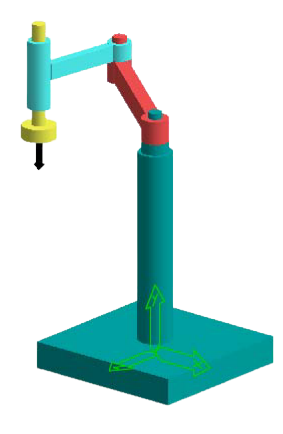
\includegraphics[trim = {0cm 0 0cm 0}, clip, height=1.5\textwidth]{scara2.png}
        \end{figure}   
    
    \end{columns}
    
%*----------- notes
    \note[item]{Tem como objetivo pose do end effector a partir dos deslocamentos angulares e lineares das juntas. Pela notação D-H é possível descrever uma junta com 4 parâmetros.}
\end{frame}
%*----------- SLIDE -------------------------------------------------------------
% \begin{frame}{Graus de Liberdade}
%     \begin{figure}
%         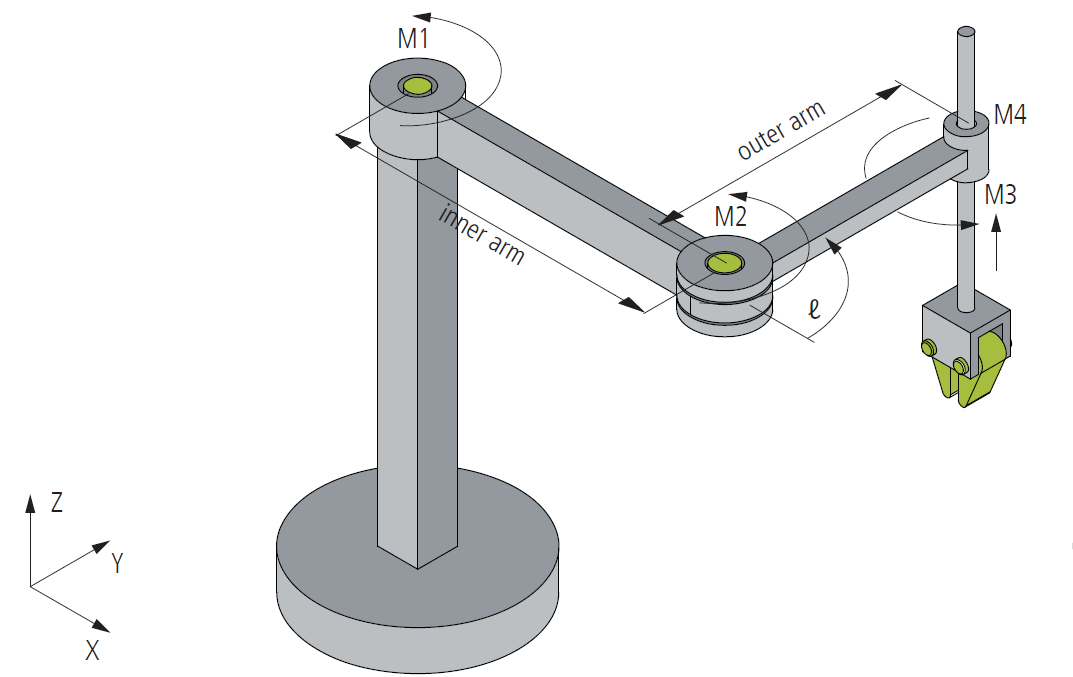
\includegraphics[trim = 160 0 0 0, clip, width=0.6\textwidth]{1232566667__Web.png}
%         %\caption{.}
%     \end{figure}     
% \end{frame}
%*----------- SLIDE -------------------------------------------------------------
\begin{frame}[c]{Cinemática Direta x Cinemática Inversa} 
    % \transdissolve[duration=0.5]

    \begin{figure}
        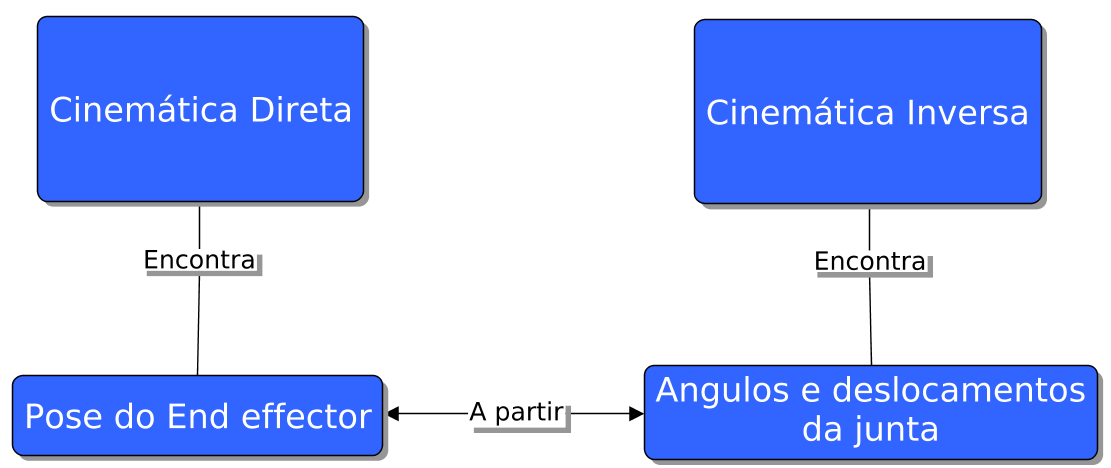
\includegraphics[trim = 0 0 0 0, clip, height=.38\textwidth]{cinematica.png}
        %\caption{.}
    \end{figure}
        
    %*----------- notes
    % \begin{center}
    %     \Wider{%
    %     \begin{shaded}
    %     \begin{center}
    %         \vspace*{0.5cm}
    %         \resizebox{!}{0.7cm}{%
    %             \textcolor{cyan}{G}\textcolor{red}{o}\textcolor{orange}{o}\textcolor{cyan}{g}\textcolor{teal}{l}\textcolor{red}{e}?
    %         }%
    %     \end{center}
    %     \end{shaded}
    %     }%
    % \end{center}
%*----------- notes
    \note[item]{Notes can help you to remember important information. Turn on the notes option.}
\end{frame}
%*----------- SLIDE -------------------------------------------------------------
\begin{frame}[c]{Cinemática Direta} 
    \framesubtitle{Notação Denavit-Hartenberg}
    Tem como objetivo obter o conjunto de equações que descreve a cinemática direta de um robô. \\
    Cada junta do robô é descrita através de 4 parâmetros:
    \begin{itemize}
        \item $\theta$ - Ângulo de rotação da junta
        \item d - Deslocamento da junta
        \item a - Comprimento do elo
        \item $\alpha$ - Ângulo de torção da junta
        
    \end{itemize}

%*----------- notes
    \note[item]{Tem como objetivo pose do end effector a partir dos deslocamentos angulares e lineares das juntas. Pela notação D-H é possível descrever uma junta com 4 parâmetros.}
\end{frame}
%*----------- SLIDE -------------------------------------------------------------
\begin{frame}[c]{Cinemática Direta} 
    \framesubtitle{Notação Denavit-Hartenberg}
    \large
    
    \begin{figure}
        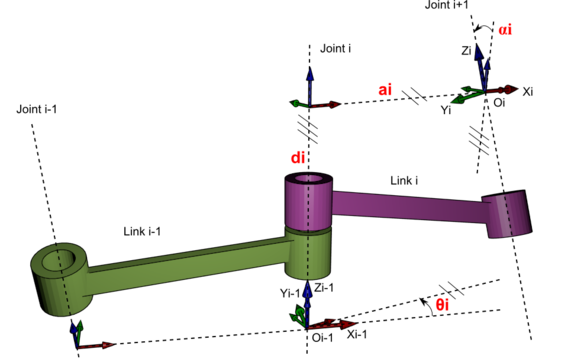
\includegraphics[trim = 0 0 0 0, clip, height=0.4\textwidth]{Classic-DHparameters.png}
    \end{figure}

%*----------- notes
    \note[item]{Tem como objetivo pose do end effector a partir dos deslocamentos angulares e lineares das juntas. Pela notação D-H é possível descrever uma junta com 4 parâmetros.}
\end{frame}
%*----------- SLIDE -------------------------------------------------------------
\begin{frame}[c]{Notação Denavit-Hartenberg} 
    % \framesubtitle{Notação Denavit-Hartenberg}
    \large
    
    \begin{figure}
        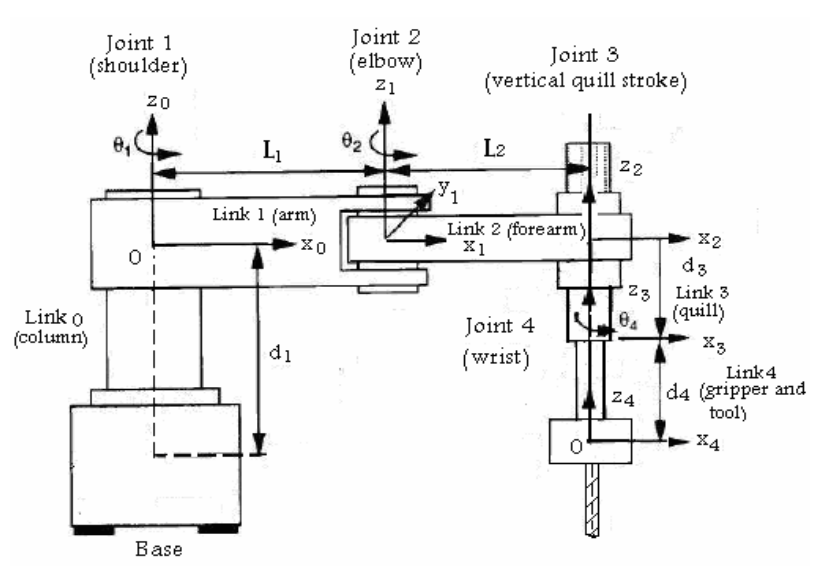
\includegraphics[trim = 0 1cm 0 0, clip, height=0.48\textwidth]{dhnota.png}
    \end{figure}

%*----------- notes
    \note[item]{Tem como objetivo pose do end effector a partir dos deslocamentos angulares e lineares das juntas. Pela notação D-H é possível descrever uma junta com 4 parâmetros.}
\end{frame}
%*----------- SLIDE -------------------------------------------------------------
\begin{frame}[c]{Notação Denavit-Hartenberg} 
    % \framesubtitle{Notação Denavit-Hartenberg}
    \large
    
    \begin{figure}
        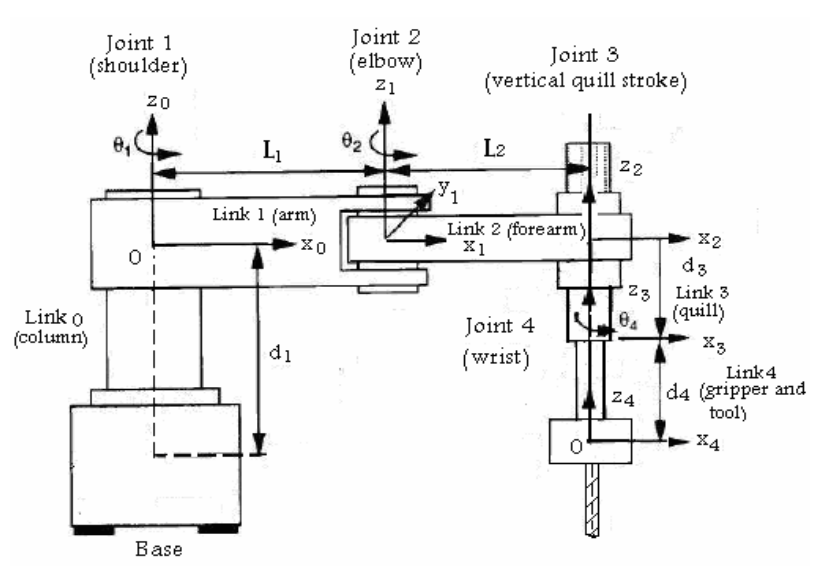
\includegraphics[trim = 0 0 0 0, clip, height=0.35\textwidth]{dhnota.png}
        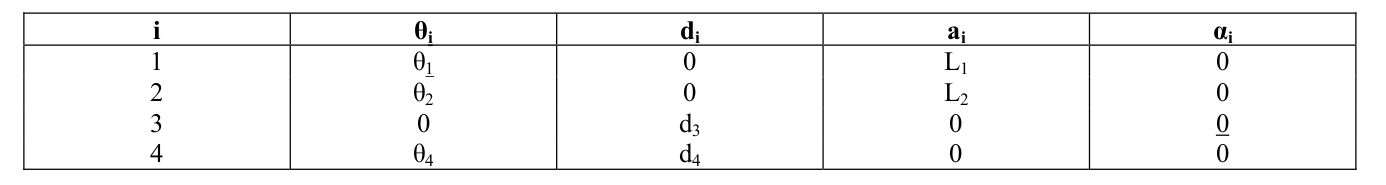
\includegraphics[trim = 0 0 0 0, clip, width=.9\textwidth]{Screenshot from 2021-11-01 18-12-13.png}
    \end{figure}
%*----------- notes
    \note[item]{Tem como objetivo pose do end effector a partir dos deslocamentos angulares e lineares das juntas. Pela notação D-H é possível descrever uma junta com 4 parâmetros.}
\end{frame}
%*----------- SLIDE -------------------------------------------------------------
\begin{frame}[c]{Notação Denavit-Hartenberg} 
    \framesubtitle{Matriz de Transformação Homogênea}
    \large{
    \begin{itemize}
        \item Matriz de transformação da junta (i-1) e i:\\
        \vspace{0.3cm}
        $T_{i}^{i-1}=Rot(z,\theta_{i})\cdot Trans(z,d_{i})\cdot Trans(x,a_{i})\cdot Rot(x,\alpha_{i})$\\
    \end{itemize}
    
    \begin{itemize}
        \item Matriz de transformação homogênea:\\
        \vspace{0.3cm}
        $T_{n}^{0}=T_{1}^{0}\cdot T_{2}^{1} \cdot T_{3}^{2} \cdots T_{n}^{n-1}$
    \end{itemize}
    }
    % 
\includegraphics[clip, trim = 0 0 0 0,  width=.83\textwidth]{databases.jpg}
%*----------- notes
    \note[item]{Tem como objetivo pose do end effector a partir dos deslocamentos angulares e lineares das juntas. Pela notação D-H é possível descrever uma junta com 4 parâmetros.}
\end{frame}
%*----------- SLIDE -------------------------------------------------------------
\begin{frame}[c]{Cinemática Inversa} 
    \large
    % \framesubtitle{Pouco tempo para muito resultado}
    % \transdissolve[duration=0.5]
    A cinemática inversa tem como objetivo encontrar deslocamentos angulares e lineares das juntas a partir da pose do end effector.\\% Normalmente para cada pose existem mais de uma solução.\\
    A matriz de transformação homemogênea é igual ao produto das matrizes de transformação de uma junta para outra:\\
    \vspace{.15cm}

    \begin{center}
        $T_{4}^{0}=T_{1}^{0}\cdot T_{2}^{1} \cdot T_{3}^{2} \cdot T_{4}^{3}$\\
    \end{center}

    \vspace{.15cm}
    Logo, solucionando para a junta 4, por exemplo:\\
    \vspace{.2cm}
    \begin{center}
        $T_{4}^{3}=(T_{3}^{2})^{-1} \cdot (T_{2}^{1})^{-1} \cdot (T_{1}^{0})^{-1} \cdot T_{4}^{0}$    
    \end{center}    
%*----------- notes
    \note[item]{Notes can help you to remember important information. Turn on the notes option.}
\end{frame}
 %*----------- SLIDE -------------------------------------------------------------
 \begin{frame}
    \begin{columns}
        %\column{.01\textwidth}
        \column{0.4\textwidth}
        ~\hfill
            \begin{beamercolorbox}[sep=8em, colsep*=18pt, wd=\textwidth,ht=\paperheight]{title page header}
                \begin{center}
                    \textbf{\huge{DINÂMICA}}\par
                \end{center}
            \end{beamercolorbox}%
            
        \column{.05\textwidth} 
        \column{.6\textwidth}
        \Large
        Para o estudo da dinâmica do robô é necessário modelar:
        \vspace{.4cm}
        \begin{itemize}
            \item Atuadores
            \item Transmissões
            \item Juntas
        \end{itemize}
    \end{columns}
  
%*----------- notes
    \note[item]{Notes can help you to remember important information. Turn on the notes option.}
 \end{frame}
 %*----------- SLIDE -------------------------------------------------------------
\begin{frame}[c]{Resultados} 
    \framesubtitle{$\theta_{1}=1.6493$ rad e $\theta_{2}=1.475-2.6178$ rad}
    \begin{columns}
        \column{0.5\textwidth}
        \begin{center}
            \Large \textbf{Matlab}\\     
        \end{center}
        \begin{figure}
            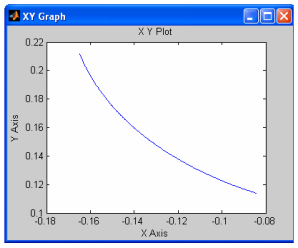
\includegraphics[trim = 0 0 0 0, clip, height=.68\textwidth]{m_1.png}
        \end{figure}
        \column{0.49\textwidth}
        \begin{center}
            \Large \textbf{SD Software}\\    
        \end{center}
        \begin{figure}
            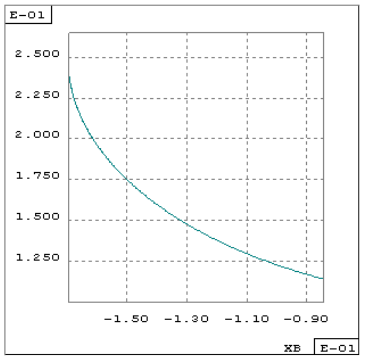
\includegraphics[trim = 0 0 0 0, clip, height=.68\textwidth]{sd_1.png}
        \end{figure}
              
    \end{columns}
\end{frame}
 %*----------- SLIDE -------------------------------------------------------------
 \begin{frame}[c]{Resultados} 
    \framesubtitle{$\theta_{1}=3.0142-0.794125$ rad e $\theta_{2}=2.4495696$ rad}
    \begin{columns}
        \column{0.5\textwidth}
        \begin{center}
            \Large \textbf{Matlab}\\    
        \end{center}
        \begin{figure}
            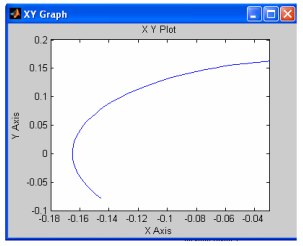
\includegraphics[trim = 0 0 0 0, clip, height=.68\textwidth]{m_2.png}
        \end{figure}
        \column{0.49\textwidth}
        \begin{center}
            \Large \textbf{SD Software}\\   
        \end{center}
        \begin{figure}
            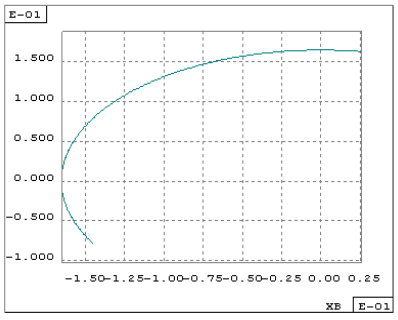
\includegraphics[trim = 0 0 0 0, clip, height=.68\textwidth]{sd_2.png}
        \end{figure}
              
    \end{columns}
\end{frame}
 %*----------- SLIDE -------------------------------------------------------------
 \begin{frame}[c]{Resultados} 
    \framesubtitle{$\theta_{1}=0.232-2.4695$ rad e $\theta_{2}=1.3521- 2.0944$ rad}
    \begin{columns}
        \column{0.5\textwidth}
        \begin{center}
            \Large \textbf{Matlab}\\    
        \end{center}
        \begin{figure}
            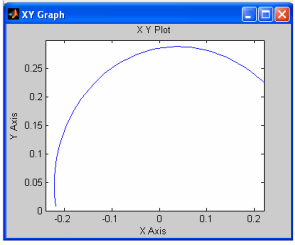
\includegraphics[trim = 0 0 0 0, clip, height=.68\textwidth]{m_3.png}
        \end{figure}
        \column{0.49\textwidth}
        \begin{center}
            \Large \textbf{SD Software}\\    
        \end{center}
        \begin{figure}
            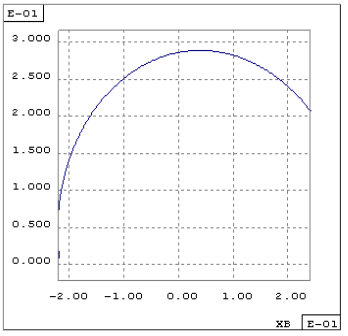
\includegraphics[trim = 0 0 0 0, clip, height=.68\textwidth]{sd_3.png}
        \end{figure}
              
    \end{columns}
\end{frame}
%*----------- SLIDE -------------------------------------------------------------
\begin{frame}[c]{Conclusão} 
\Large
\begin{itemize}
    \item Foi desenvolvido um completo modelo matemático
    \item As equações de cinemática direta e inversa foram obtidas através da notação de Danevit-Hartenberg
    \item Foram feitas simulações em Matlab e Solid Dynamics Software
    \item Os resultados de ambos softwares foram concordantes
\end{itemize}
\end{frame}

% \begin{frame}[c]{teste}
%     \begin{center}
%         \Wider{%
%         \begin{shaded}
%         \begin{center}
%             \vspace*{0.5cm}
%             \resizebox{!}{5cm}{%
%             \begin{figure}
%                 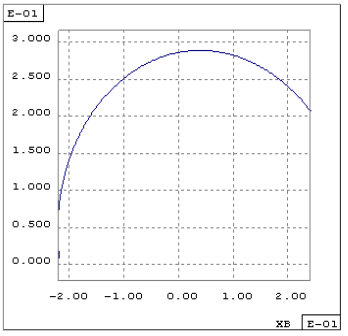
\includegraphics[trim = 0 0 0 0, clip, height=1\textwidth]{sd_3.png}
%             \end{figure}    
%             % \textcolor{cyan}{G}\textcolor{red}{o}\textcolor{orange}{o}\textcolor{cyan}{g}\textcolor{teal}{l}\textcolor{red}{e}?
%             }%
%         \end{center}
%         \end{shaded}
%         }%
%     \end{center}
% \end{frame}[c]{teste}

